\chapter{PHÂN TÍCH HỆ THỐNG}
\label{ch:system-analysis}

\section{Use Case Diagram}
\label{sec:use-case-diagram}

\subsection{Tổng quan Use Case}
\label{subsec:use-case-overview}

Hệ thống DSA Visualizer Platform phục vụ ba nhóm actor chính: Student, Instructor và Admin. Mỗi actor có các use case riêng biệt phù hợp với vai trò và quyền hạn của họ trong hệ thống.

\begin{figure}[H]
\centering
\includegraphics[width=0.9\textwidth]{enhanced-diagrams/usecase-main-system.png}
\caption{Use Case Diagram tổng quan của hệ thống}
\label{fig:main-usecase}
\end{figure}

\subsection{Use Case chi tiết cho Learning Process}
\label{subsec:learning-process-usecase}

Quá trình học tập là core functionality của platform, bao gồm nhiều use case phức tạp với các interaction giữa Student và các subsystem khác nhau.

\begin{figure}[H]
\centering
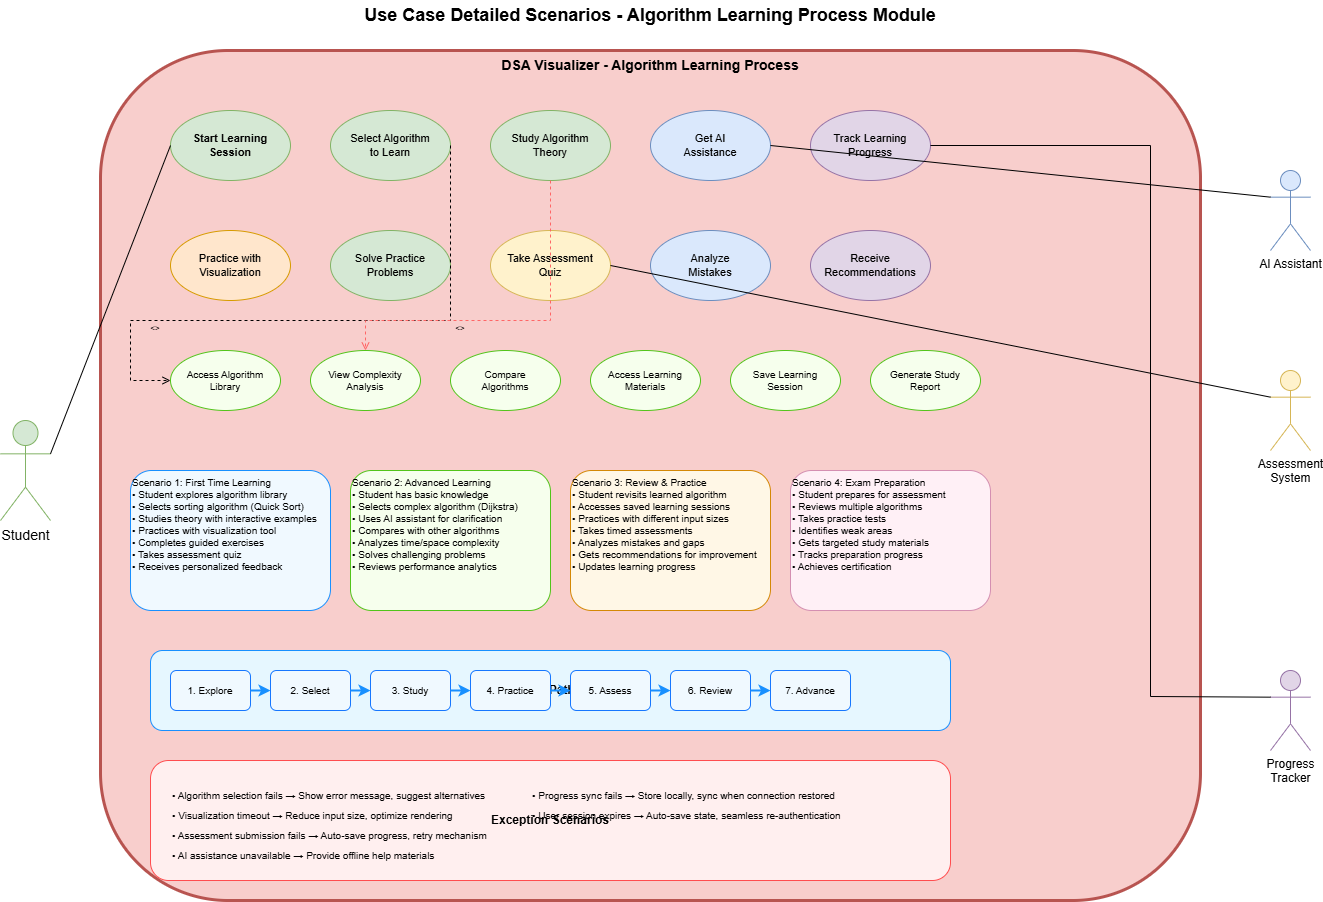
\includegraphics[width=1.0\textwidth]{enhanced-diagrams/usecase-detailed-scenarios.png}
\caption{Use Case Diagram chi tiết cho Algorithm Learning Process}
\label{fig:learning-usecase}
\end{figure}

Các use case chính trong Learning Process:

\begin{enumerate}
    \item \textbf{Start Learning Session}: Khởi tạo session học tập mới
    \item \textbf{Select Algorithm}: Chọn thuật toán cần học
    \item \textbf{Study Theory}: Đọc tài liệu lý thuyết
    \item \textbf{Practice with Visualization}: Thực hành với animation
    \item \textbf{Solve Practice Problems}: Giải bài tập thực hành
    \item \textbf{Take Assessment}: Làm bài kiểm tra đánh giá
    \item \textbf{Get AI Assistance}: Nhận hỗ trợ từ AI assistant
    \item \textbf{Track Progress}: Theo dõi tiến độ học tập
\end{enumerate}

\subsection{Detailed Use Case Specifications}
\label{subsec:detailed-usecase-specs}

\subsubsection{Use Case: Practice with Visualization}

\begin{table}[H]
\centering
\caption{Mô tả Use Case: Practice with Visualization}
\label{tab:uc-practice-visualization}
\begin{tabularx}{\textwidth}{|l|X|}
\hline
\textbf{Use Case ID} & UC-VIS-001 \\ \hline
\textbf{Use Case Name} & Practice with Visualization \\ \hline
\textbf{Actor} & Student \\ \hline
\textbf{Description} & Student tương tác với visualizer để hiểu cách thuật toán hoạt động từng bước \\ \hline
\textbf{Preconditions} & 
- Student đã đăng nhập vào hệ thống \\
- Student đã chọn thuật toán cần học \\ \hline
\textbf{Postconditions} & 
- Visualization history được lưu vào learning progress \\
- Time spent tracking được cập nhật \\ \hline
\textbf{Main Flow} & 
1. Student truy cập visualization page \\
2. System hiển thị thuật toán với default input \\
3. Student có thể: \\
\hspace{0.5cm} 3.1. Thay đổi input data \\
\hspace{0.5cm} 3.2. Điều chỉnh animation speed \\
\hspace{0.5cm} 3.3. Step through từng bước \\
\hspace{0.5cm} 3.4. View synchronized code \\
4. Student click "Start Animation" \\
5. System chạy visualization với settings đã chọn \\
6. Student quan sát và học tập \\
7. System lưu progress và statistics \\ \hline
\textbf{Alternative Flows} & 
A1: Custom Input \\
\hspace{0.5cm} 3.1a. Student nhập custom input \\
\hspace{0.5cm} 3.1b. System validate input format \\
\hspace{0.5cm} 3.1c. Nếu invalid: show error message \\
\\
A2: AI Assistance \\
\hspace{0.5cm} 6.1a. Student click "Get Help" \\
\hspace{0.5cm} 6.1b. AI Assistant explain current step \\
\hspace{0.5cm} 6.1c. Continue with main flow \\ \hline
\textbf{Exception Flows} & 
E1: Animation Error \\
\hspace{0.5cm} 5.1a. Animation fails to render \\
\hspace{0.5cm} 5.1b. System show error message \\
\hspace{0.5cm} 5.1c. Offer alternative visualization mode \\ \hline
\end{tabularx}
\end{table}

\subsubsection{Use Case: Get AI Assistance}

\begin{table}[H]
\centering
\caption{Mô tả Use Case: Get AI Assistance}
\label{tab:uc-ai-assistance}
\begin{tabularx}{\textwidth}{|l|X|}
\hline
\textbf{Use Case ID} & UC-AI-001 \\ \hline
\textbf{Use Case Name} & Get AI Assistance \\ \hline
\textbf{Actor} & Student \\ \hline
\textbf{Description} & Student nhận hỗ trợ từ AI assistant để hiểu thuật toán hoặc giải quyết vấn đề \\ \hline
\textbf{Preconditions} & 
- Student đã đăng nhập vào hệ thống \\
- AI service available \\ \hline
\textbf{Postconditions} & 
- Conversation history được lưu \\
- AI usage statistics được cập nhật \\ \hline
\textbf{Main Flow} & 
1. Student click "AI Assistant" button \\
2. System mở AI chat interface \\
3. Student nhập câu hỏi hoặc chọn suggested questions \\
4. System gửi request đến AI service với context \\
5. AI service process request và trả về response \\
6. System hiển thị AI response với formatting \\
7. Student có thể: \\
\hspace{0.5cm} 7.1. Tiếp tục hỏi follow-up questions \\
\hspace{0.5cm} 7.2. Request code examples \\
\hspace{0.5cm} 7.3. Ask for explanation in different language \\
8. System lưu conversation history \\ \hline
\textbf{Alternative Flows} & 
A1: Code Generation Request \\
\hspace{0.5cm} 3.1a. Student request code for current algorithm \\
\hspace{0.5cm} 3.1b. Student chọn programming language \\
\hspace{0.5cm} 4.1a. AI generate code với explanation \\
\hspace{0.5cm} 6.1a. System hiển thị syntax-highlighted code \\
\\
A2: Step-by-step Explanation \\
\hspace{0.5cm} 3.2a. Student click "Explain Current Step" \\
\hspace{0.5cm} 4.2a. AI explain current visualization step \\
\hspace{0.5cm} 6.2a. Explanation synchronized với animation \\ \hline
\textbf{Exception Flows} & 
E1: AI Service Unavailable \\
\hspace{0.5cm} 4.1a. AI service timeout hoặc error \\
\hspace{0.5cm} 4.1b. System show fallback static help \\
\hspace{0.5cm} 4.1c. Log error for admin notification \\
\\
E2: Rate Limit Exceeded \\
\hspace{0.5cm} 4.2a. Too many requests from user \\
\hspace{0.5cm} 4.2b. System show rate limit message \\
\hspace{0.5cm} 4.2c. Suggest waiting period \\ \hline
\end{tabularx}
\end{table}

\section{Class Diagram}
\label{sec:class-diagram}

\subsection{Core Domain Classes}
\label{subsec:core-classes}

Hệ thống được thiết kế theo Domain-Driven Design với các core domain classes sau:

\begin{figure}[H]
\centering
\includegraphics[width=1.0\textwidth]{diagrams/class-diagram-core.png}
\caption{Class Diagram cho Core Domain}
\label{fig:class-core}
\end{figure}

\subsubsection{User Management Classes}

\begin{itemize}
    \item \textbf{User}: Base class cho tất cả users
    \item \textbf{Student}: Extends User, thêm learning-specific attributes
    \item \textbf{Instructor}: Extends User, thêm teaching-specific attributes  
    \item \textbf{Admin}: Extends User, thêm system management capabilities
\end{itemize}

\subsubsection{Learning Domain Classes}

\begin{itemize}
    \item \textbf{Algorithm}: Represents thuật toán với metadata
    \item \textbf{Visualization}: Chứa animation data và configuration
    \item \textbf{LearningSession}: Tracks user interaction với algorithm
    \item \textbf{Progress}: Theo dõi learning progress của user
    \item \textbf{Assessment}: Quiz và evaluation system
\end{itemize}

\subsection{Service Layer Classes}
\label{subsec:service-classes}

\begin{figure}[H]
\centering
\includegraphics[width=1.0\textwidth]{diagrams/class-diagram-services.png}
\caption{Class Diagram cho Service Layer}
\label{fig:class-services}
\end{figure}

\subsubsection{Visualization Services}

\begin{itemize}
    \item \textbf{VisualizationEngine}: Core engine cho animation rendering
    \item \textbf{AnimationController}: Điều khiển animation playback
    \item \textbf{DataProcessor}: Xử lý input data cho visualization
    \item \textbf{RenderingService}: Abstract layer cho different renderers
\end{itemize}

\subsubsection{AI Services}

\begin{itemize}
    \item \textbf{AIAssistant}: Main interface cho AI interactions
    \item \textbf{OpenAIService}: Integration với OpenAI GPT
    \item \textbf{GeminiService}: Integration với Google Gemini
    \item \textbf{ContextBuilder}: Xây dựng context cho AI requests
\end{itemize}

\section{Activity Diagram}
\label{sec:activity-diagram}

\subsection{Learning Process Flow}
\label{subsec:learning-flow}

Activity diagram sau mô tả complete learning process từ khi student bắt đầu học một thuật toán mới:

\begin{figure}[H]
\centering
\includegraphics[width=0.8\textwidth]{diagrams/activity-learning-process.png}
\caption{Activity Diagram cho Learning Process}
\label{fig:activity-learning}
\end{figure}

\subsubsection{Main Activities}

\begin{enumerate}
    \item \textbf{Algorithm Selection}: Student chọn thuật toán từ library
    \item \textbf{Theory Study}: Đọc theoretical background
    \item \textbf{Visualization Practice}: Tương tác với animated visualization
    \item \textbf{Code Understanding}: Phân tích implementation code
    \item \textbf{Problem Solving}: Áp dụng thuật toán vào bài tập
    \item \textbf{Assessment}: Đánh giá mức độ hiểu biết
    \item \textbf{Progress Update}: Cập nhật learning progress
\end{enumerate}

\subsubsection{Decision Points}

\begin{itemize}
    \item \textbf{Prerequisite Check}: Kiểm tra điều kiện tiên quyết
    \item \textbf{Difficulty Assessment}: Đánh giá độ khó phù hợp
    \item \textbf{Understanding Verification}: Xác nhận mức độ hiểu
    \item \textbf{Need Help Decision}: Quyết định có cần AI assistance
\end{itemize}

\subsection{AI Assistance Flow}
\label{subsec:ai-flow}

\begin{figure}[H]
\centering
\includegraphics[width=0.7\textwidth]{diagrams/activity-ai-assistance.png}
\caption{Activity Diagram cho AI Assistance Flow}
\label{fig:activity-ai}
\end{figure}

Process khi student request AI help:

\begin{enumerate}
    \item \textbf{Context Collection}: Gather current learning context
    \item \textbf{Query Processing}: Process natural language query
    \item \textbf{AI Model Selection}: Chọn appropriate AI model
    \item \textbf{Response Generation}: Generate contextual response
    \item \textbf{Response Formatting}: Format cho display
    \item \textbf{Feedback Collection}: Thu thập user feedback
\end{enumerate}

\section{Sequence Diagram}
\label{sec:sequence-diagram}

\subsection{Visualization Rendering Sequence}
\label{subsec:visualization-sequence}

Sequence diagram sau mô tả interaction giữa các components khi render visualization:

\begin{figure}[H]
\centering
\includegraphics[width=1.0\textwidth]{diagrams/sequence-visualization.png}
\caption{Sequence Diagram cho Visualization Rendering}
\label{fig:sequence-viz}
\end{figure}

\subsubsection{Participants}

\begin{itemize}
    \item \textbf{Student}: User initiating visualization
    \item \textbf{VisualizationUI}: Frontend visualization component
    \item \textbf{VisualizationEngine}: Core rendering engine
    \item \textbf{AnimationController}: Animation management
    \item \textbf{DataProcessor}: Input data processing
    \item \textbf{ProgressTracker}: Learning progress tracking
\end{itemize}

\subsubsection{Key Interactions}

\begin{enumerate}
    \item Student selects algorithm và input parameters
    \item UI validates input và sends request to engine
    \item Engine processes data và prepares animation steps
    \item AnimationController manages playback timing
    \item Progress tracking updates throughout process
    \item Final state saved to user progress
\end{enumerate}

\subsection{AI Assistant Interaction Sequence}
\label{subsec:ai-sequence}

\begin{figure}[H]
\centering
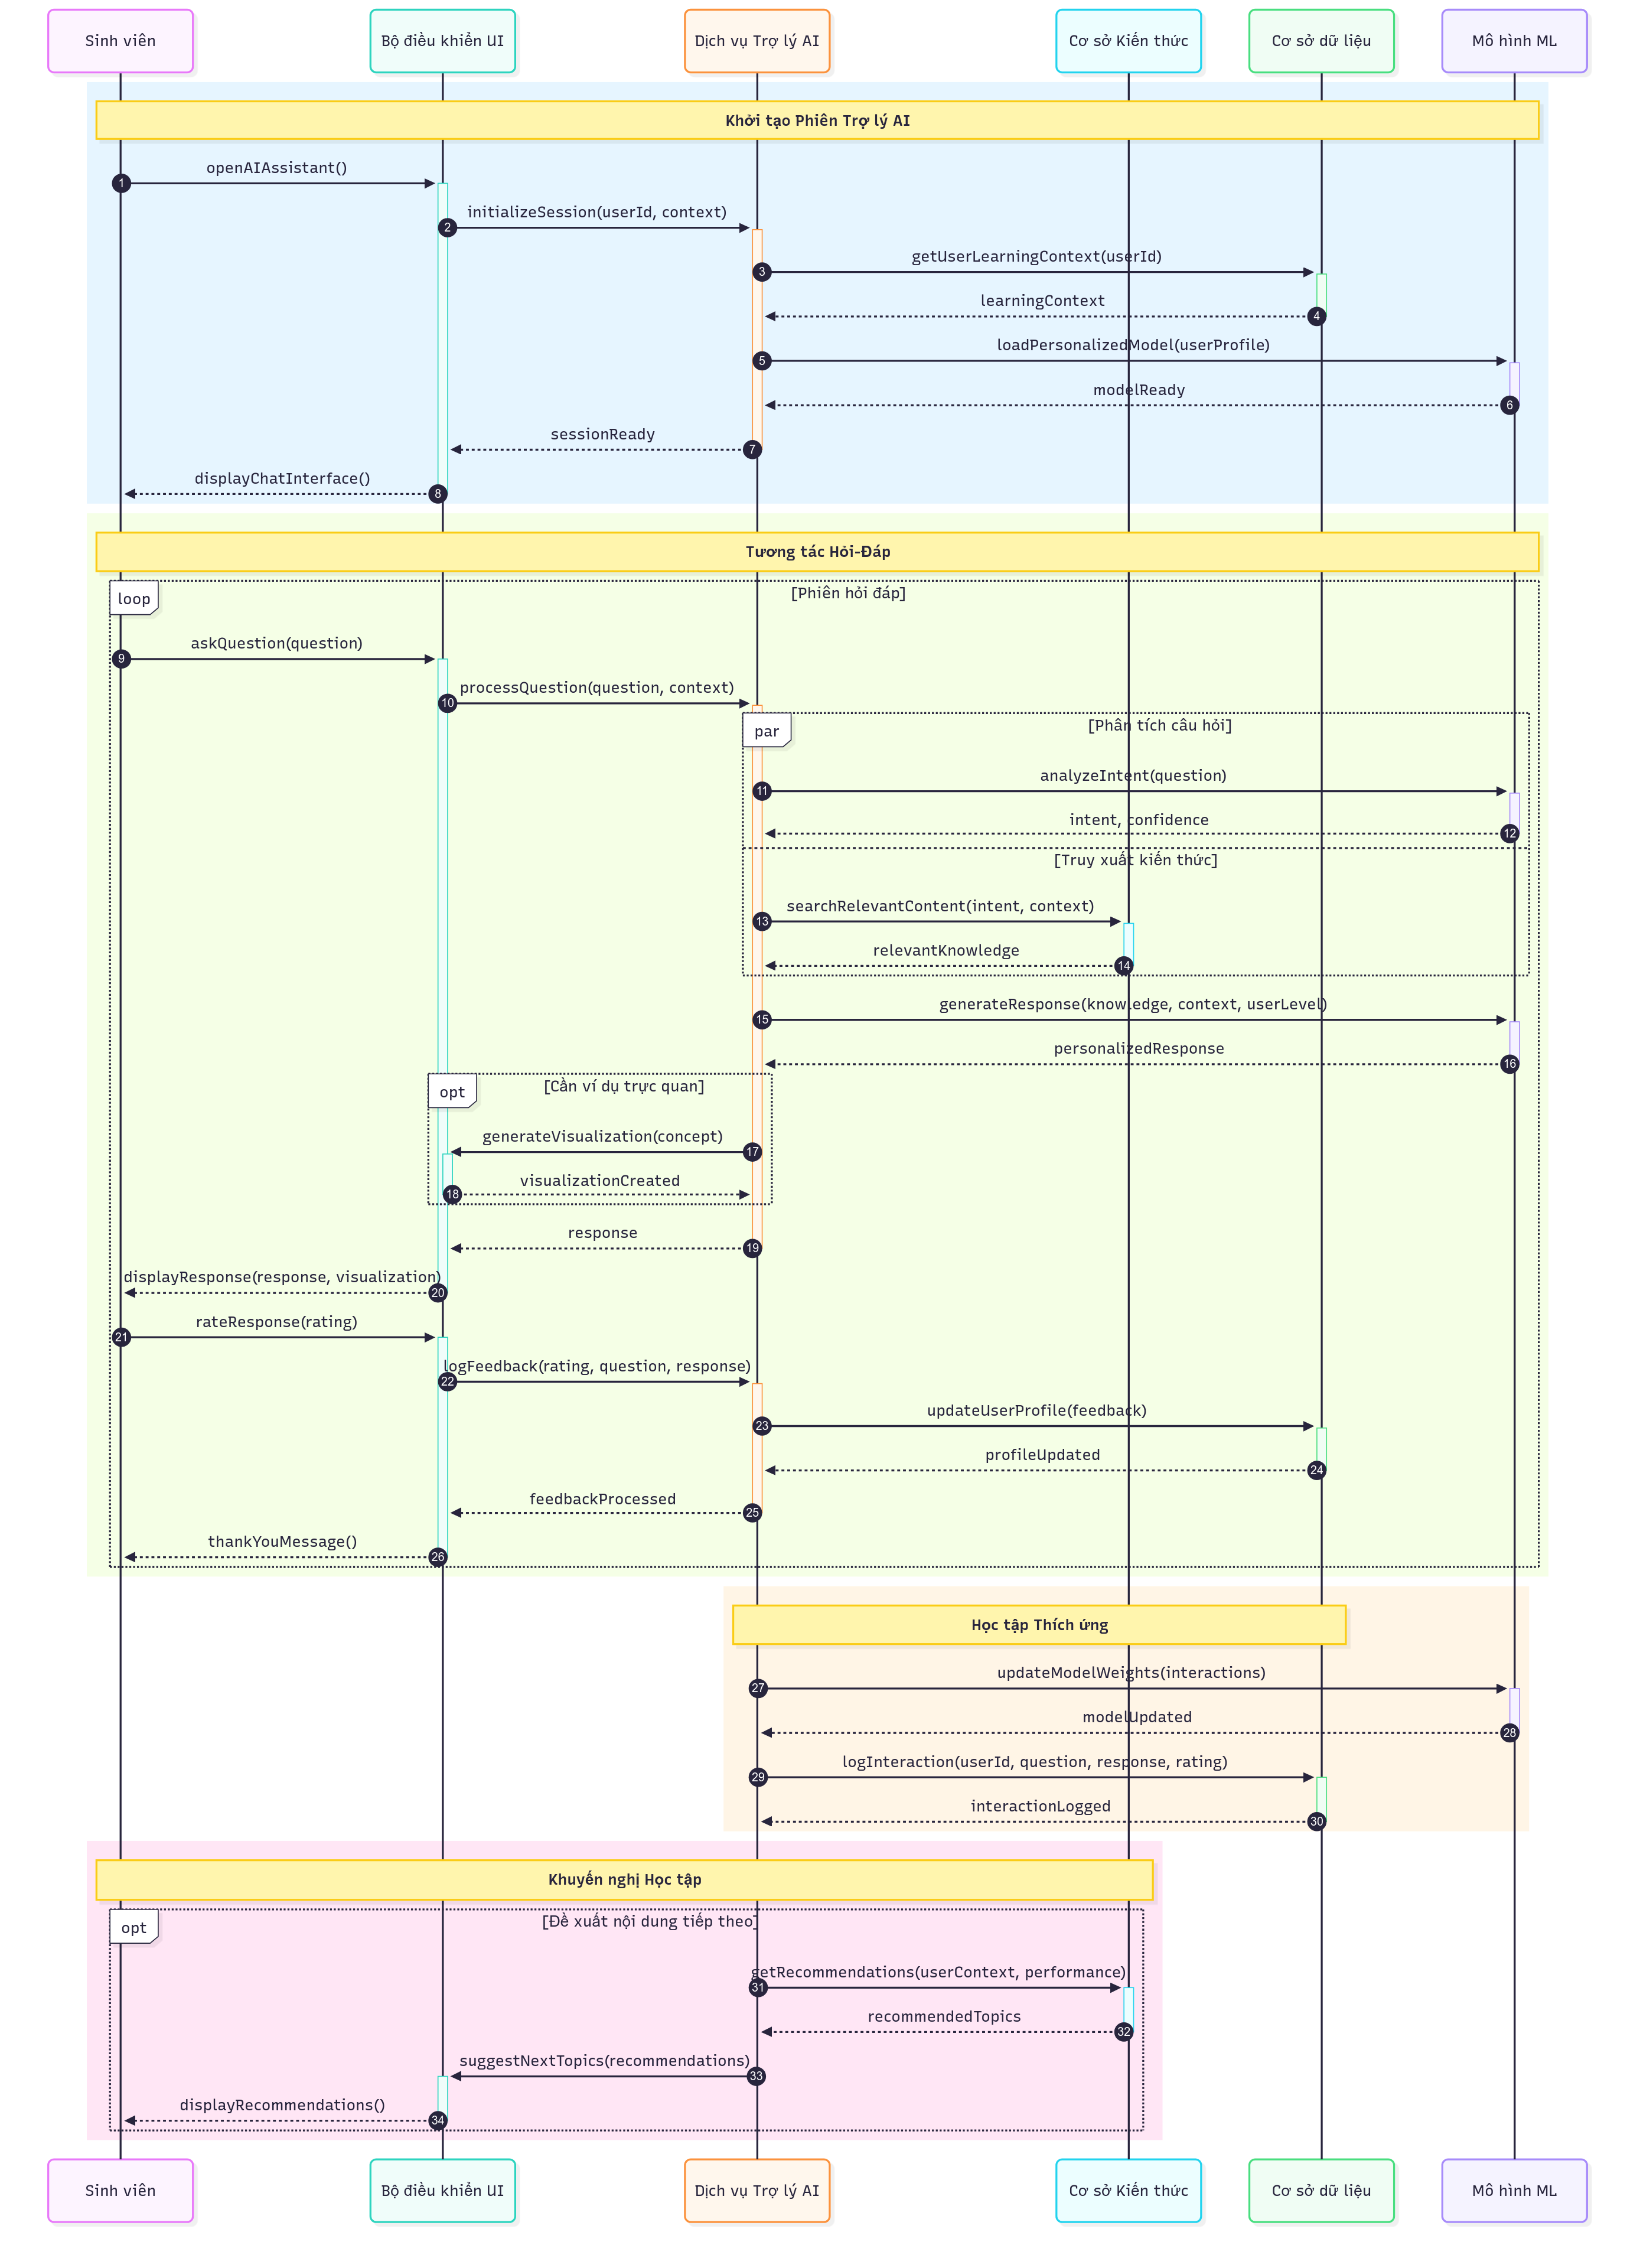
\includegraphics[width=1.0\textwidth]{diagrams/sequence-ai-assistant.png}
\caption{Sequence Diagram cho AI Assistant Interaction}
\label{fig:sequence-ai}
\end{figure}

\subsubsection{Multi-Model AI Architecture}

Platform sử dụng multiple AI models để optimize cho different use cases:

\begin{enumerate}
    \item \textbf{OpenAI GPT}: Cho natural language explanations
    \item \textbf{Google Gemini}: Cho code generation và analysis
    \item \textbf{Context Router}: Intelligent routing dựa trên query type
    \item \textbf{Response Aggregator}: Combine responses từ multiple models
\end{enumerate}

\subsection{Community Interaction Sequence}
\label{subsec:community-sequence}

\begin{figure}[H]
\centering
\includegraphics[width=1.0\textwidth]{diagrams/sequence-community.png}
\caption{Sequence Diagram cho Community Features}
\label{fig:sequence-community}
\end{figure}

Mô tả interaction trong forum và Q\&A system:

\begin{enumerate}
    \item User posts question hoặc discussion topic
    \item System validates content và applies moderation rules
    \item Notification service alerts relevant users
    \item Other users provide answers và comments
    \item Voting system ranks responses
    \item AI assistant có thể provide supplementary answers
    \item Final resolution updates knowledge base
\end{enumerate}
